% THIS IS SIGPROC-SP.TEX - VERSION 3.1
% WORKS WITH V3.2SP OF ACM_PROC_ARTICLE-SP.CLS
% APRIL 2009
%
% It is an example file showing how to use the 'acm_proc_article-sp.cls' V3.2SP
% LaTeX2e document class file for Conference Proceedings submissions.
% ----------------------------------------------------------------------------------------------------------------
% This .tex file (and associated .cls V3.2SP) *DOES NOT* produce:
%       1) The Permission Statement
%       2) The Conference (location) Info information
%       3) The Copyright Line with ACM data
%       4) Page numbering
% ---------------------------------------------------------------------------------------------------------------
% It is an example which *does* use the .bib file (from which the .bbl file
% is produced).
% REMEMBER HOWEVER: After having produced the .bbl file,
% and prior to final submission,
% you need to 'insert'  your .bbl file into your source .tex file so as to provide
% ONE 'self-contained' source file.
%
% Questions regarding SIGS should be sent to
% Adrienne Griscti ---> griscti@acm.org
%
% Questions/suggestions regarding the guidelines, .tex and .cls files, etc. to
% Gerald Murray ---> murray@hq.acm.org
%
% For tracking purposes - this is V3.1SP - APRIL 2009

\documentclass{edm_template}
\usepackage{multirow}
\usepackage{csquotes}
\usepackage{listings}
\usepackage{fixltx2e}
\usepackage{floatrow}
\usepackage{url}
\usepackage{mathtools}
\usepackage[font=small,skip=0pt]{caption}

\makeatletter
\def\@copyrightspace{\relax}
\makeatother
\setlength{\floatsep}{5pt}
\setlength{\textfloatsep}{4pt}
\setlength{\intextsep}{5pt}

\newcommand{\squishlist}{
 \begin{list}{$\bullet$}
 {
  \setlength{\itemsep}{0pt}
  \setlength{\parsep}{3pt}
  \setlength{\topsep}{3pt}
  \setlength{\partopsep}{0pt}
  \setlength{\leftmargin}{1.5em}
  \setlength{\labelwidth}{1em}
  \setlength{\labelsep}{0.5em} } }

\newcommand{\squishlisttwo}{
 \begin{list}{$\bullet$}
 {
  \setlength{\itemsep}{0pt}
  \setlength{\parsep}{0pt}
  \setlength{\topsep}{0pt}
  \setlength{\partopsep}{0pt}
  \setlength{\leftmargin}{2em}
  \setlength{\labelwidth}{1.5em}
  \setlength{\labelsep}{0.5em} } }

\newcommand{\squishend}{
  \end{list}  }

\begin{document}

\title{Portrait of an Indexer---Computing Pointers Into Instructional Videos}
%\subtitle{[Extended Abstract]
%\titlenote{A full version of this paper is available as
%\textit{Author's Guide to Preparing ACM SIG Proceedings Using
%\LaTeX$2_\epsilon$\ and BibTeX} at
%\texttt{www.acm.org/eaddress.htm}}}
%
% You need the command \numberofauthors to handle the 'placement
% and alignment' of the authors beneath the title.
%
% For aesthetic reasons, we recommend 'three authors at a time'
% i.e. three 'name/affiliation blocks' be placed beneath the title.
%
% NOTE: You are NOT restricted in how many 'rows' of
% "name/affiliations" may appear. We just ask that you restrict
% the number of 'columns' to three.
%
% Because of the available 'opening page real-estate'
% we ask you to refrain from putting more than six authors
% (two rows with three columns) beneath the article title.
% More than six makes the first-page appear very cluttered indeed.
%
% Use the \alignauthor commands to handle the names
% and affiliations for an 'aesthetic maximum' of six authors.
% Add names, affiliations, addresses for
% the seventh etc. author(s) as the argument for the
% \additionalauthors command.
% These 'additional authors' will be output/set for you
% without further effort on your part as the last section in
% the body of your article BEFORE References or any Appendices.

\numberofauthors{4} %  in this sample file, there are a *total*
% of EIGHT authors. SIX appear on the 'first-page' (for formatting
% reasons) and the remaining two appear in the \additionalauthors section.
%
\author{
% You can go ahead and credit any number of authors here,
% e.g. one 'row of three' or two rows (consisting of one row of three
% and a second row of one, two or three).
%
% The command \alignauthor (no curly braces needed) should
% precede each author name, affiliation/snail-mail address and
% e-mail address. Additionally, tag each line of
% affiliation/address with \affaddr, and tag the
% e-mail address with \email.
%
% 1st. author
\alignauthor Andrew Lamb \\
       \affaddr{Stanford University} \\
       \email{andrew.lamb@stanford.edu }
\alignauthor Jose Hernandez \\
       \affaddr{Stanford University} \\
       \email{josehdz@stanford.edu }
\alignauthor Jeffrey Ullman \\
       \affaddr{Stanford University} \\
       \email{ullman@cs.stanford.edu }
\and
\alignauthor Andreas Paepcke \\
       \affaddr{Stanford University} \\
       \email{paepcke@cs.stanford.edu}
% \and   use '\and' if you need 'another row' of author names
} % \author
\date{9 February 2016}
% Just remember to make sure that the TOTAL number of authors
% is the number that will appear on the first page PLUS the
% number that will appear in the \additionalauthors section.

\maketitle
% Probably put in a little bit more.
\begin{abstract}
We examine algorithms for creating indexes into ordered series of
instructional lecture video transcripts. The goal is for students and
industry practitioners to use the indexes towards review or
reference. Lecture videos differ from often-examined document
collections such as newspaper articles in that the transcript ordering
generally reflects pedagogical intent. One challenge is therefore to
identify where a concept is {\em primarily} introduced, and where the
resulting index should thus direct students. The typically applied
TF-IDF approach gets tricked in this context by artifacts such as
worked examples whose associated vocabulary may dominate a lecture,
but should not be included in a good index. We contrast the TF-IDF
approach with algorithms that consult Wikipedia documents to vouch for
term importance. This method helps filter the harmful artifacts. We
measure the algorithms against three human-created indexes over the 90
lecture videos of a popular database course. We found that {\em (i)}
humans have low inter-rater reliability, whether they are experts in
the field or not, and that {(\em ii)} one of the examined algorithms
approaches the inter-rater reliability with humans.
\end{abstract}

%% A category with the (minimum) three required fields
%\category{H.4}{Information Systems Applications}{Miscellaneous}
%%A category including the fourth, optional field follows...
%\category{D.2.8}{Software Engineering}{Metrics}[complexity measures, performance measures]
%
%\terms{Theory}

\section{Introduction}
\label{sec:intro}

Offerings of massively open online courses (MOOCs) have been expanding
over the past years. Companies are betting their existence on the
continuation of this trend. Universities are experimenting to find
their own approaches, either to teaching open classes, or to develop
courses directed to their enrolled students. Thus, while the embrace
of the `massive,' and `open' portions of MOOCs might vary, the
`online' aspect as a tool for teaching is gaining ground, and we focus
on this aspect here. Best practices for the use of the Internet to
teach are still evolving, and not all voices are enthusiastic
\cite{Eckerdal2014}. Nonetheless, given the trend it is essential to
develop technologies that take maximum advantage of the online medium.

Current course offerings expose many opportunities for such
technologies. Peer assessment, forum use, guided tutoring, and
interventions that address dropout rates all offer such possibilities
for technological improvement \cite{Piech2013,
  balfour2013,Coetzee2014, agrawal2015, halawa2014dropout,
  yang2013turn}.

We focus here on opportunities arising when students need to review
course material before approaching assessments. Other intended
beneficiaries of this work are industrial practitioners wishing to
learn parts of course material.  Course reviews are historically
offered by instructors to peers of students. In online settings,
however, students may not arrive at courses on traditional term
boundaries; so students' review time lines are not aligned as they
would be among a fixed group of peers. In the extreme,
\textit{untended} courses may not have any active teaching
staff. Without support, students fend for themselves when they don't
understand a concept or need to review for a test.

One important source for students to review in today's online courses
are lecture videos. Typical courses include 100 or more such
presentations. While the sequential nature of video may make them
suited for structured, linear pedagogy during concept introductions,
their sequentiality is clumsy when videos are used as reference
material during course review activities. For those occasions random
access as afforded by the traditional index at the end of books is
much more appropriate. We are not proposing a student-facing {\em
  interface} that mimics book indexes; we are rather referring to the
{\em capabilities} of book indexes---however they can best manifest in
online teaching.

The problem is that human indexing is very expensive. We therefore
present comparisons of algorithms that can be applied towards the
automatic production of indexes into instructional videos. We use as
our raw material the closed caption files that are often available for
educational video. Those files contain transcripts of the videoed
instructor's words, paired with timing information at roughly sentence
granularity.

The challenge in effective indexing is that keywords must not only
reference the important elements of concepts, and must furthermore
direct students to the video segments that contain the {\em primary}
treatments of those concepts. Competent indexing into instructional
videos can serve as the foundation to a number of higher-level
facilities for students. In \cite{agrawal2015} we discussed how
answers to forum post questions might be approached using video
indexes. Other opportunities include automated advice for review when
students struggle with particular assignments, and facilities that
make courses suitable as reference resources for professionals after
they complete a course.

Many keyword extraction systems are designed for use on large
collections of loosely related documents, such as newspaper articles
\cite{Salton1975}, or are directed at summarizing or indexing
individual documents \cite{ohsawa1998}.

In contrast, the algorithms we study here are confronted with a series
of video transcript files that introduce a number of related concepts
in pedagogically thought-through order. Many keyword extraction
algorithms leverage the fact that documents on very different topics
will have mostly disjoint sets of words, which may not be the case in
our setting where very few authors (i.e. instructors) produce all the
documents.

Evaluation of an algorithm's success in building a `good' index is
particularly difficult because indexing from free text is a highly
subjective process. We do not in this work operate with pre-defined
keyword sets from which an algorithm would choose. Instead, the harder
task we set for our algorithms is freely to choose words from the text
that should be included in the index, subject possibly to a stemming
process. The task thus holds many degrees of freedom that allow for a
multitude of outcomes.

Given this lack of a natural ground truth, we decided to evaluate
outcomes for our algorithms by comparing against decisions made by
humans. We paid three humans to carefully index the video transcripts
from a Stanford online database course.  We examined how well the
three resulting indexes compared to each other, and how outcomes of
several algorithms compared to each of the human-generated results. We
make the three reference indexes and the database course video caption
files available to the public in hope of eliciting indexing approaches
beyond those that we explored.

Figure~\ref{fig:task} is a schematic of the task solved by the human
and algorithmic indexers.
\begin{figure}[htp]
       \centering
       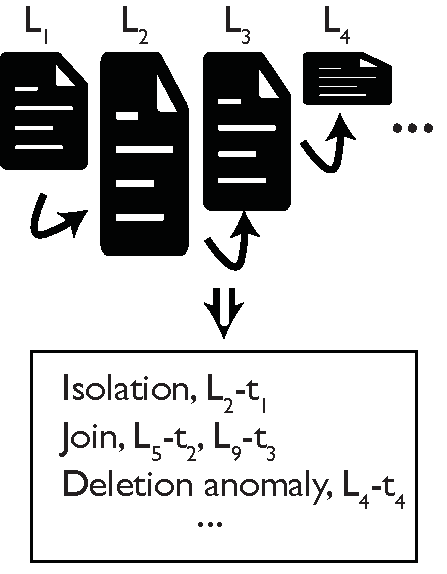
\includegraphics[height=2in]{indexingTask.pdf}
       \caption{\textnormal{The task to be solved by the algorithms
           and human indexers. Construct an index into ordered video
           lecture transcripts such that index keywords and phrases
           reference the lecture portions where corresponding concepts
           are introduced.}}
       \label{fig:task}
\end{figure}

The ordered lecture transcripts $L_1$--$L_n$ contain lines of
instructor speech, together with timing information. An index is to be
constructed that maps concept-bearing words and phrases to
lecture-time pairs. Note that index entries may map to multiple
lectures, if the corresponding word or phrase is important in those
lectures. Our current implementations set $t_n$ to the first
occurrence of the respective index term in the lecture.
Note as well that we do not impose a controlled vocabulary for the
index entries. All entries are taken from the transcript text. Any
word or phrase is therefore a potential candidate for inclusion in the
index. 

Our first experiment took a traditional approach, selecting words for
the index that appeared disproportionately often in certain
lectures. We then incorporated lexical information, by only
considering phrases that followed certain part-of-speech
patterns. Finally, we introduced external knowledge from Wikipedia
into an algorithm's indexing decisions. Note that none of the
algorithms included supervised learning, as we do not assume the
existence of a training set for all courses.

In Section~\ref{sec:relWork} we review some of the related
literature. Section~\ref{sec:gold} offers more detail on how we
created our three human-generated reference
indexes. Section~\ref{sec:exp} introduces the algorithms we
explored. Section~\ref{sec:discussion} offers some observations around
the experimental results, and we conclude in a final section.


%% This task of forming an index over the lectures in an online course,
%% which we refer to as the keyword extraction task, is inherently
%% difficult. A human performing the task must have a deep understanding
%% of the concepts in each lecture, as well as their role in the broader
%% context of the entire course. A 25 minute lecture video might have
%% around 4500 individual words, from which the algorithm must form
%% around 20 phrases to capture the content of the lecture. There is a
%% certain amount of subjectivity inherent in the task, and there can be
%% differing reasonable interpretations of what should be considered a
%% keyword. When humans select important phrases from a lecture they use
%% previous knowledge - for example, in a databases course one might use
%% previous knowledge of functional dependencies to decide that
%% ``Armstrong's Axiom'' should be one of the keyphrases - and we draw on
%% this strategy to automatically decide on keyphrases.



\section{Related Work}
\label{sec:relWork}

\section{Preparation of Gold Index}
\label{sec:gold}

% Describe how we had the index prepared: Paid workers, the course,
% instructions they received. Some stats: average number of index terms
% they came up with, inter-rater reliability.

In order to evaluate our algorithms, we prepared a gold standard index
of terms extracted from an introductory databases course by three paid
human indexers. Each was presented with all ~90 course closed caption
video transcripts, and was asked to work through each file in the
order the videos were presented in class. Videos were usually around
10 minutes long.

From each line in a file the indexers were asked to select as many
keywords and phrases as they felt should appear in their
index. Indexers were only allowed to use words or phrases that
appeared in the text. They were asked not to generate their own
original phrases. We used indexers' selected keywords and phrases in
our investigation\footnote{From here on we use the term `phrase' to
  mean n-grams of any length, including one, unless the distinction is
  significant.}. Additionally we asked indexers for two more pieces of
information that we did not use, but which are included in our public
copies of the indexers' results.

First, we asked indexers also to mark lines in which a particular
phrase for the index appeared in the context of the primary
introduction to the phrase's underlying concept.  Second, for each
lecture file, indexers ranked the top five most important phrases from
that lecture. We allowed inclusion of fewer than five phrases.

One participant had taken the database course being indexed. A second
indexer had taken at least one database course in another institution,
and the third was a college-educated individual in a non-technical
field.

On average indexers selected about 8 phrases per video.  We evaluated
agreement between the indexers' output using Fleiss' Kappa, which
generalizes Cohen's Kappa to settings with more than two annotators
\cite{fleiss1971measuring}. The $\kappa$ is a measure of inter-rater
agreement, with range $[-1, 1]$, where 1 means the raters are in
complete agreement, -1 complete disagreement, and 0 the agreement
expected by chance.

For our algorithms we formulate the indexing problem as a binary
classification task, where the two categories are {\em in-index} and
{\em not-in-index}. The algorithms' task was to classify phrases in
each lecture into these two buckets.

%% Specifically, we have the algorithms classify phrases that are either
%% 1-grams or have been tagged as an {\em in-index} phrase by at least one
%% rater. For example, in the sentence `One of them is what's called
%% the inner join on a condition', where `inner join' has been marked as
%% a keyword, the algorithms will be evaluated on their classification
%% of `inner join' and `condition', but not on the phrase `one of'.
% Given a set of raters and a collection of lectures $\ell_1, \ldots,
% \ell_n$, where each lecture contains phrases $p_1, \ldots, p_n \in
% \ell_i$, we define the set of examples as the set of lecture-phrase
% pairs $(\ell, p)$ such that $p$ appears in $\ell$, and $p$ is either a
% 1-gram or $(\ell, p)$ was tagged as an {\em in-index} phrase by at
% least one rater.

When not comparing against each of the three indexers individually, we
combined the work of all three into a single index by computing the
lecture-by-lecture three-way union. Several other approaches for
combining the three ground truth examples can be formulated. We
selected the union because it was the most licentious for the
algorithms. However, when comparing algorithm results to individual
indexers the respective indexer's actual work was used.

We computed a $\kappa$ of 0.325 between the indexes produced by the
three human raters. This $\kappa$ is evidence of significant
differences between the decisions of the three indexers. The
non-expert was much more prolific in choosing {\em in-index} phrases
than the two experts. But even the two experts frequently made
different choices.

We consider this $\kappa$ the upper bound on the performance we could
reasonably expect from any indexing algorithm. The largest pairwise
Cohen's $\kappa$ between raters was 0.336 and the lowest was 0.309
(note that Fleiss' Kappa is not generally the average of the pairwise
Cohen's Kappas).

\section{Experiments}
\label{sec:exp}

% Introduce what we are trying to do: explore different methods for
% building the index, and comparing against gold. Foreshadow the
% methods: naive/pedagogy-inclusive/external-knowledge.

% List whatever is common to the three experiments: stop word removal,
% method used for stemming...

We implemented different keyword extraction algorithms and measured how closely they agreed with the gold index formed by human annotators.

% Insert something about the metric once we have it really nailed down.

For each experiment we apply the Porter stemming algorithm to each word in the document and each word in a keyphrase, so there will be a match between phrases if all of the individual stemmed tokens match. In experiments using n-grams as candidate phrases, stopwords were removed from the document before the n-grams were formed, using the stopword list used in the SMART system \cite{salton1971smart}. 
% In experiments using part-of-speech tagging, the Stanford Log-Linear POS tagger was used \cite{toutanova2003feature}.

\subsection{Naive Approach: TF-IDF}
\label{sec:tfidf}

Simply discard sequencing information of terms occurrences. For each
video put the top-n tf/idf terms into the index \cite{mann2008}.

\subsection{Leveraging Linguistic Information}
\label{sec:useTime}

% Do we have any experiments that do take the positions of terms in the
% sequence of videos into account? Such an experiment would nicely tell
% a story from naive TF/IDF to including pedagogy to including external
% wikipedia.

Considering all of the n-grams in the collection of lectures as
candidate keywords has the potential of adding significant noise. By
selecting only certain linguistic patterns for consideration as
phrases, it is possible to reduce the size of the candidate set, while
still covering most important phrases. We experimented with an
algorithm that first runs a part-of-speech tagger over the lecture
transcripts, and then selected only phrases that consist of an
arbitrary number of adjectives followed by one or more nouns. For
example, ``equality condition'' or ``XML data'' were both included in
the candidate set. We then ran TF-IDF over this reduced set. After
this process we proceeded as in Section~\ref{sec:tfidf}.

\subsection{Adding External Knowledge}
\label{sec:wiki}

% All of the wikipedia inclusion work.

Note that phrases gain importance because of both their role in a
document but also from their semantic meaning in the broader world.
Variants of our next algorithms therefore integrate Wikipedia as a
knowledge source.

\subsubsection{Boosting Documents}

The first variant concatenates to each lecture a closely related
Wikipedia page, and then uses the techniques of
Section~\ref{sec:useTime} to choose phrases for the index. For
example, lecture title ``View Modifications Using Triggers'', yields
as the first Wikipedia result a page titled ``Database trigger.''
This page is appended to the lecture transcript. Using either
n-grams or adjective-noun phrases as candidate keywords, the algorithm
chooses phrases with TF-IDF over the combined document for the index.

\begin{figure}
\caption{The Document Boosting algorithm searches for a Wikipedia page using the title of the lecture, concatenates the result to the lecture, and then runs TF-IDF over the combined document.}
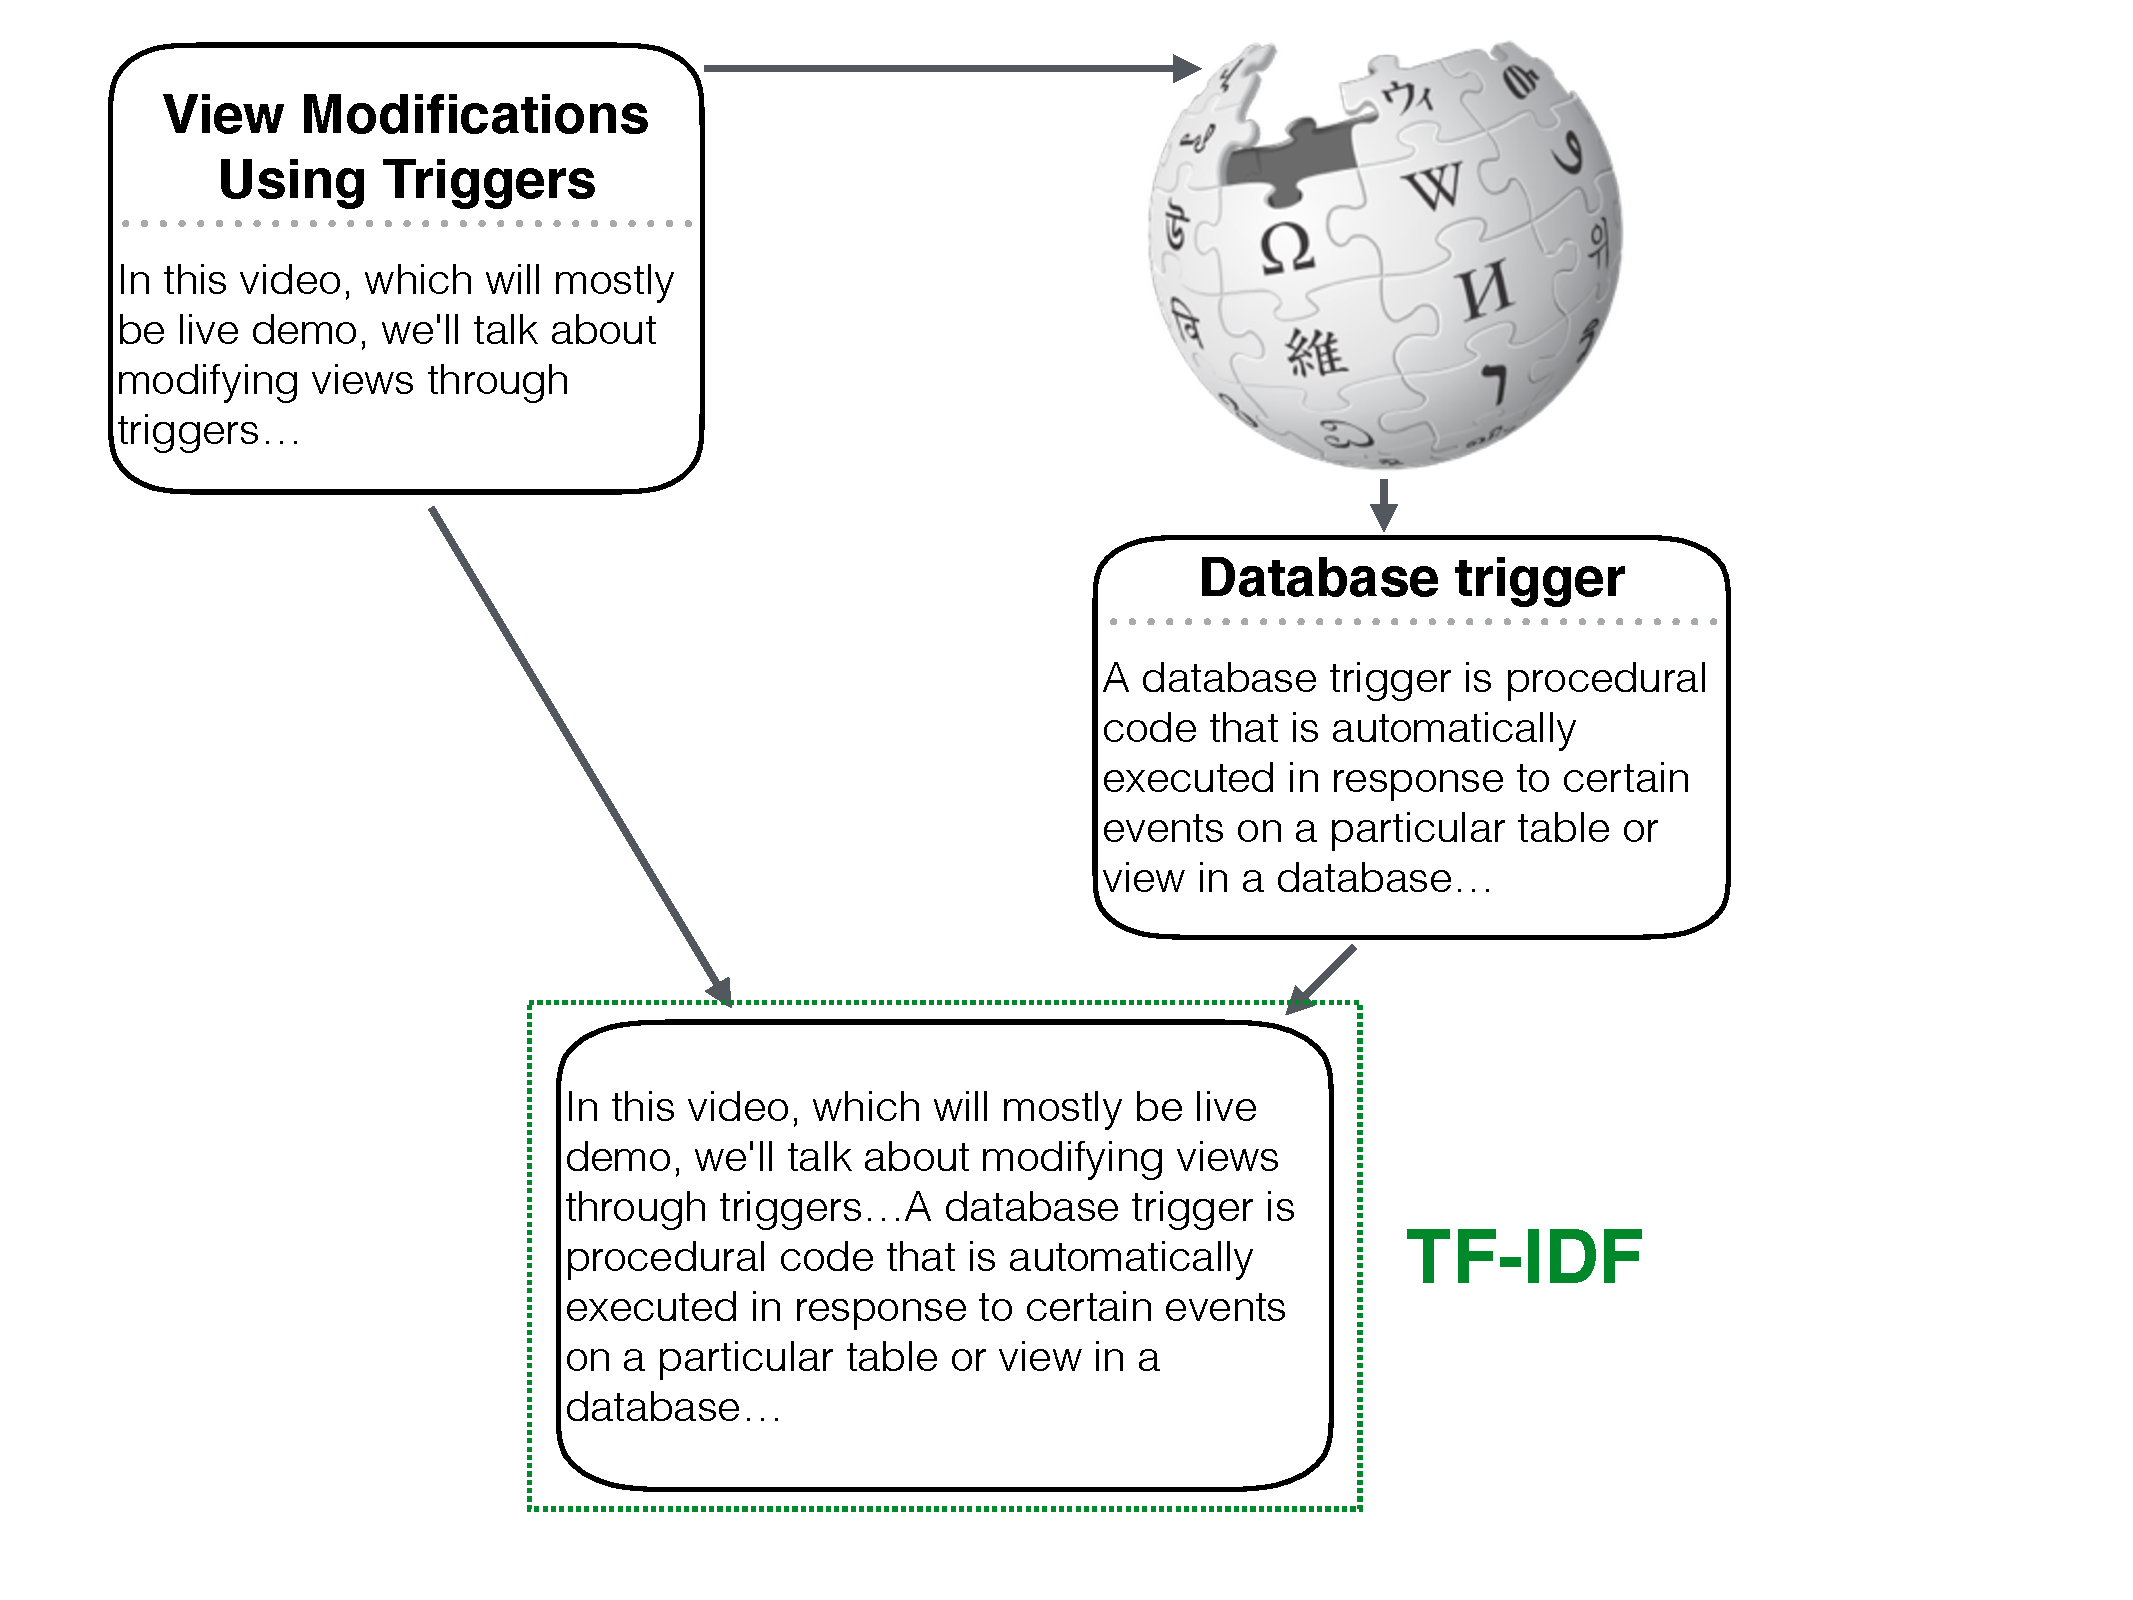
\includegraphics[width=\textwidth]{document_boosting.pdf}
\end{figure}

\subsubsection{Boosting Phrases}

This algorithm first creates a list of candidate index terms using
adjective-noun phrases. These candidates are ranked by their TF-IDF score
summed over {\bf all} Wikipedia documents.

Next, this global candidate ranking is combined with a basic TF-IDF
approach to form a final score that combines global knowledge (from
Wikipedia) with local knowledge (from the specific lecture video).
%
% First, we create a normalized Wikipedia candidate ranking
% \begin{equation*}
% TF\text{-}IDF_{w-norm}(p, W) \coloneqq \frac{TF\text{-}IDF_w(p, W)}{\sum_{p'} TF\text{-}IDF_w(p', W)}
% \end{equation*}
% and normalized lecture collection ranking
% \begin{equation*}
% TF\text{-}IDF_{norm}(p, l, L) \coloneqq \frac{TF\text{-}IDF(p, l, L)}{\sum_{p'} TF\text{-}IDF(p', l, L)}
% \end{equation*}
% Then, we combine the two normalized rankings to form a final score
% \begin{multline*}
% TF\text{-}IDF_{combined}(p, l, L, W) \coloneqq \\ \eta TF\text{-}IDF_{w-norm}(p, W) + TF\text{-}IDF_{norm}(p, l, L)
% \end{multline*}
% where $\eta$ is used to determine the weight between Wikipedia scores
% and lecture scores.

We also experimented with only boosting phrases of at least two words,
based on the intution that longer phrases are often meaningful, but
appear infrequently and are therefore given low scores by TF-IDF. We
call this alternative ``Phrase Boosting N-Grams'' in Figure
\ref{fig:main_result}.

\begin{figure}[!htbp]
\caption{The top 15 keywords from `Materialized Views' by Phrase
  Boosting with N-grams. Phrases that also appear in the gold index are marked in bold.}
\label{fig:top_15}
\begin{tabular}{|l|l|}
\hline
Rank & Phrase \\
\hline
1 & \textbf{view} \\
\hline
2 & \textbf{materialized view} \\
\hline
3 & materialized \\
\hline
4 & \textbf{query} \\
\hline
5 & \textbf{view query} \\
\hline
6 & \textbf{virtual view} \\
\hline
7 & \textbf{modify} \\
\hline
8 & user query \\
\hline
9 & \textbf{base table} \\
\hline
10 & \textbf{modify command} \\
\hline
11 & \textbf{index} \\
\hline
12 & insert command \\
\hline
13 & multivalued dependency \\
\hline
14 & \textbf{database design} \\
\hline
15 & user \\
\hline
\end{tabular}
\end{figure}

%
% A few subtleties deserve further description. First, in our simple
% TF-IDF approach, a score is calculated for each lecture $l$ and phrase
% $p$, while in our Wikipedia calculation a score is only calculated for
% each $p$. That approach is chosen because in this algorithm we are not interested in
% keywords for every Wikipedia document, but only in obtaining a global sense
% of the importance of a phrase. The algorithm is equivalent to summing over all
% Wikipedia documents $d \in W$
% \begin{equation*}
% TF_w(p) = \log \left(\sum_{d \in W} \text{number of times } p \text{ appears in } d\right)
% \end{equation*}
%
% Second, we take the logarithm of the phrase count in the Wikipedia
% ranking. This choice produces improved empirical results.
%
% \begin{figure}
% \caption{The Phrase Boosting algorithm runs TF-IDF over the entirety of Wikipedia and then combines the global ranking with a local ranking for a document.}
% 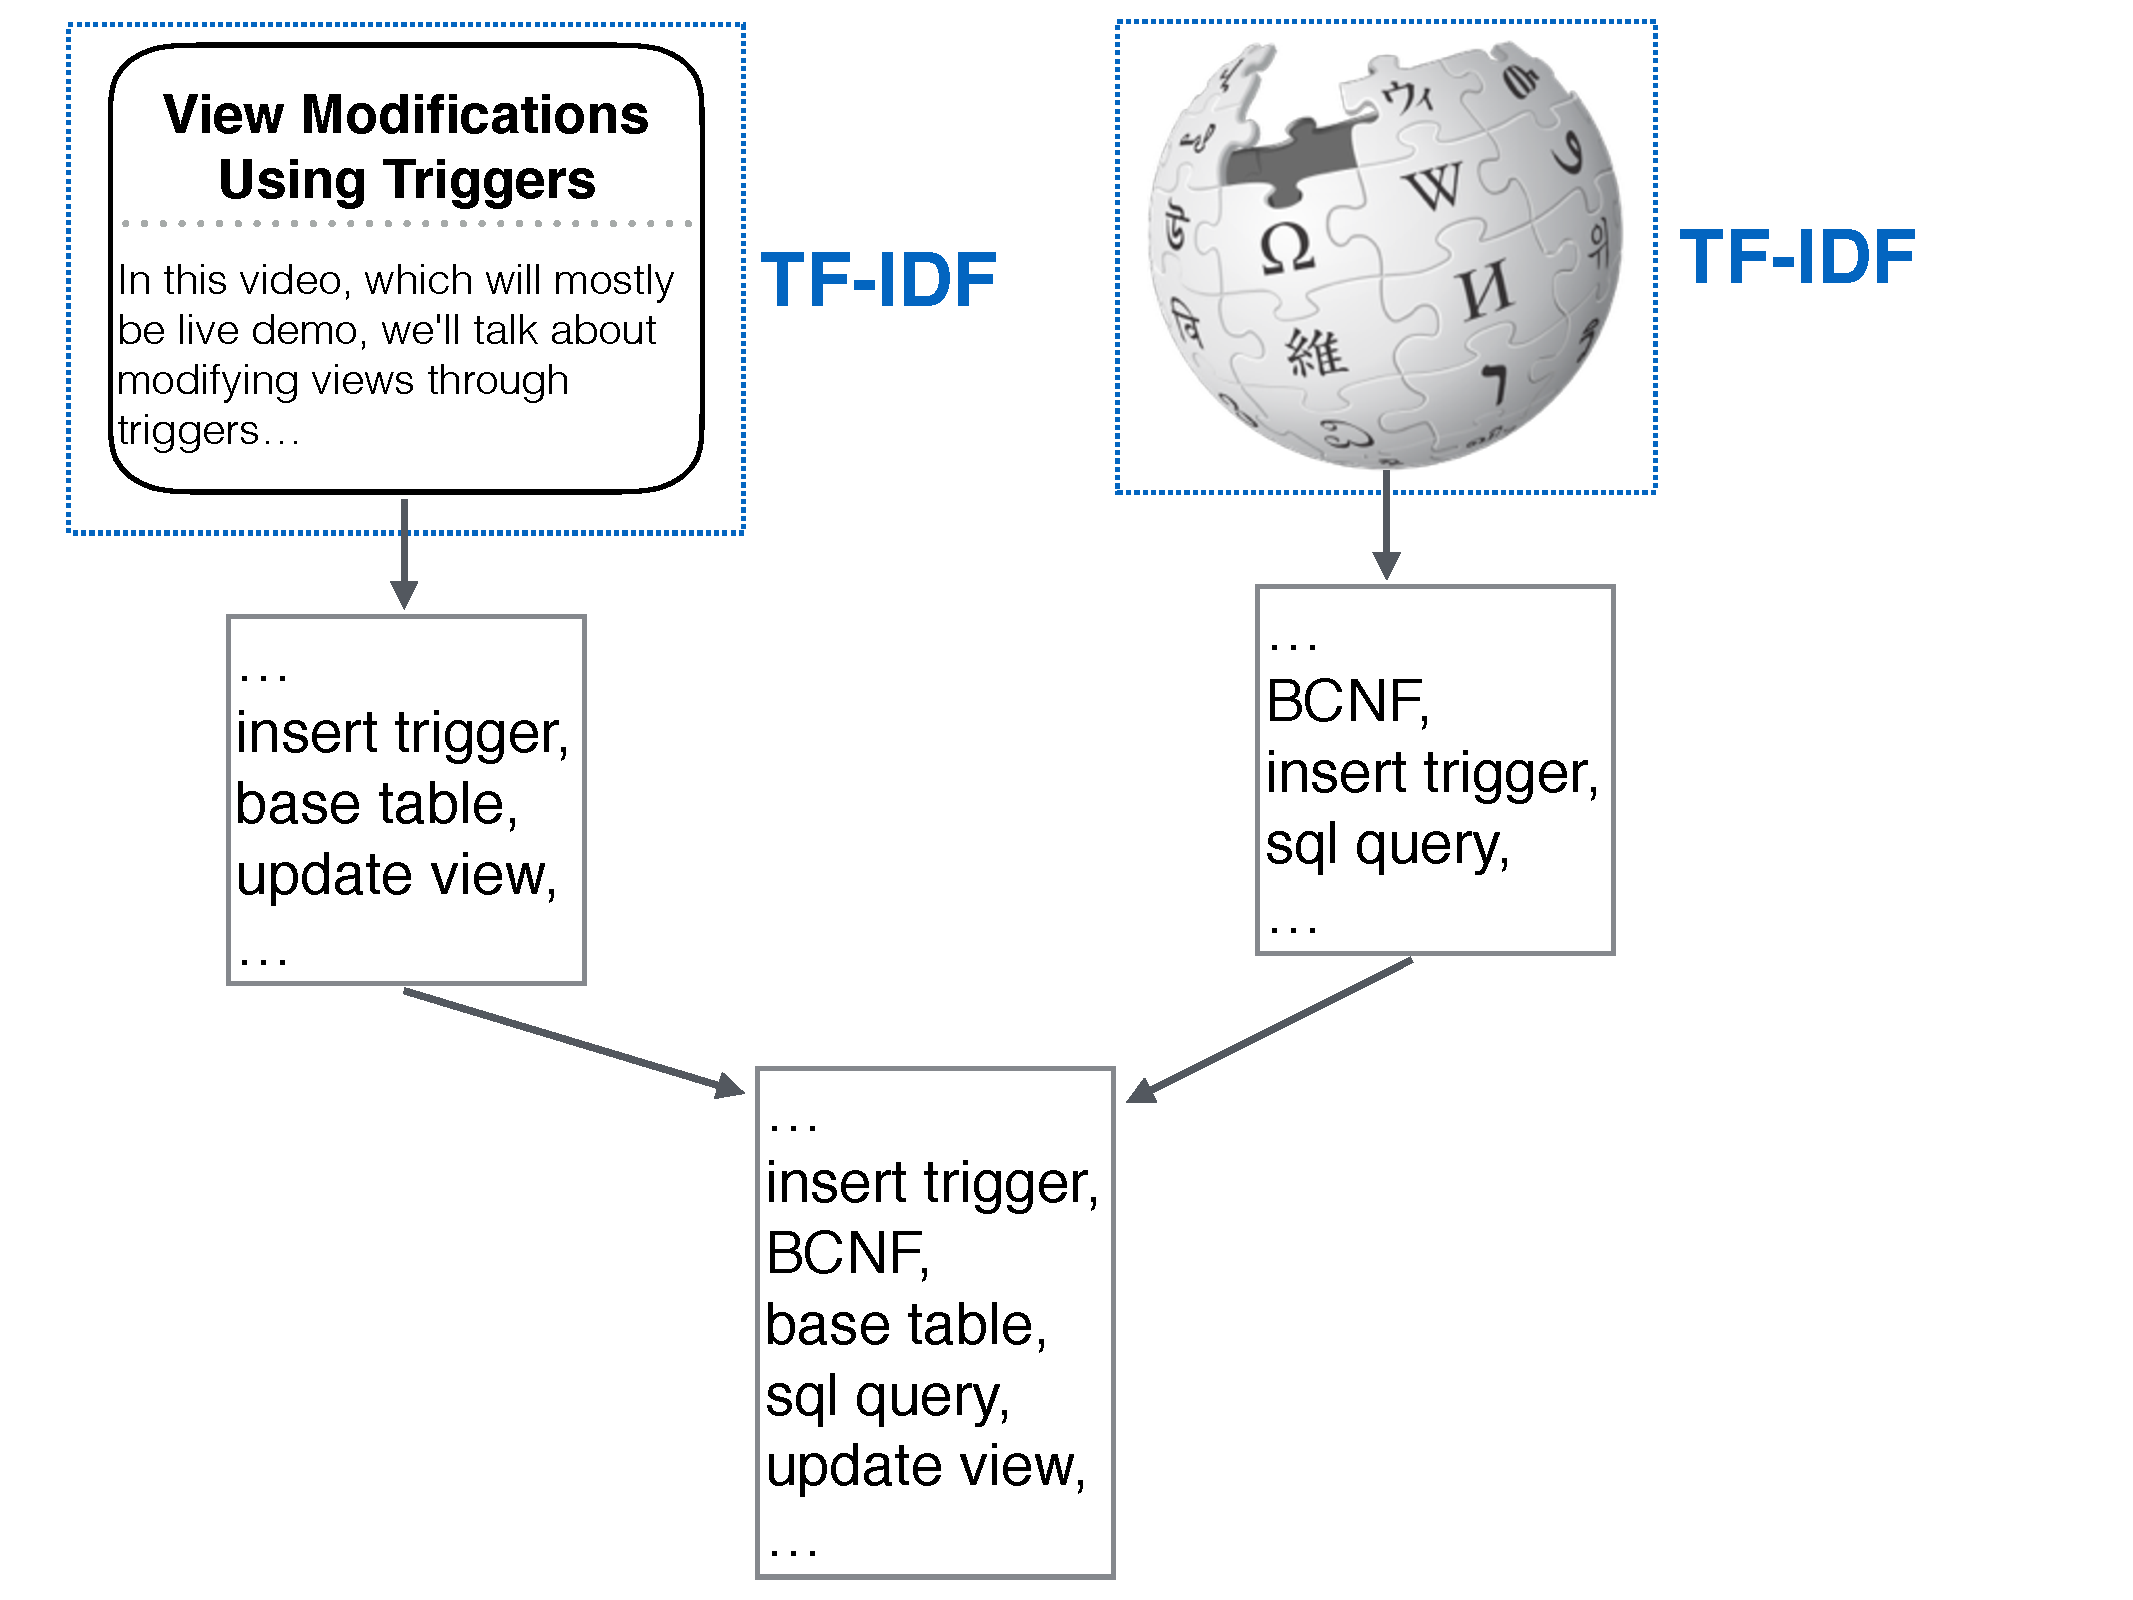
\includegraphics[width=\textwidth]{phrase_boosting.pdf}
% \end{figure}

\subsection{Summary of Results}
\label{sec:sum}

% Here is where the comparisons between the two/three experimental
% results happens.


\begin{figure*}[!ht]
\caption{}
\label{fig:main_result}
\begin{tabular}{|c|c|c|c|c|}
\hline
\textbf{Algorithm} & $\mathbf{\kappa}$ & $\mathbf{P_{\text{pos}}}$ & $\mathbf{P_{\text{neg}}}$ & \textbf{PABAK} \\
\hline
TF-IDF & 0.178 & 0.200 & 0.973 & 0.896 \\
\hline
TF-IDF with Adjective-Noun Chunks & 0.084 & 0.114 & 0.968 & 0.875 \\
\hline
Document Boosting & 0.180 & 0.199 & 0.974 & 0.901 \\
\hline
Document Boosting with Adjective-Noun Chunks & 0.131 & 0.154 & 0.971 & 0.890 \\
\hline
Phrase Boosting & 0.180 & 0.203 & 0.973 & 0.895 \\
\hline
Phrase Boosting N-Grams & \textbf{0.204} & \textbf{0.224} & \textbf{0.975} & \textbf{0.902} \\
\hline
\end{tabular}
\end{figure*}

As stated in Section~\ref{sec:gold}, we computed agreement between
humans using Fleiss' Kappa. We evaluated each algorithm by computing
Cohen's Kappa agreement between the algorithm and the gold set
unified from the three human indexes as described in
Section~\ref{sec:gold}: the union of the lecture-phrase pairs in the
gold indexes. That is a lecture-phrase pair is classified as {\em
  in-index} if any human indexer classified it as {\em in-index}, and
classified as {\em not-in-index} otherwise. When using a single metric
for agreement, such as Cohen's Kappa, paradoxes can arise when one
category is much more prevalent than another and the chance-correction
term in the agreement metric overcompensates. This effect leads to
inappropriately low values of $\kappa$ for high inter-rater agreement
\cite{feinstein1990high}.

In our case, there are many more {\em not-in-index} phrases than
phrases destined for the index. To illuminate the above-mentioned
inappropriate $\kappa$ values, we report three additional metrics:
agreement on {\em in-index} decisions ($P_{\text{pos}}$), agreement on
{\em not-in-index} decisions ($P_{\text{neg}}$)
\cite{cicchetti1990high}, and prevalence-adjusted bias-adjusted
$\kappa$ (PABAK) \cite{byrt1993bias}. Because the algorithms produce a
ranking of candidate phrases, we produce a binary classification by
choosing a threshold above which candidates are labeled as {\em
  in-index}. In our reported results, we use the average number of
keywords per lecture labeled by humans as the threshold.

These three metrics are defined in terms of a concordance table with
two raters (the composite-human and the algorithm) and two
categories ({\em in-index} and {\em not-in-index})

\begin{figure}[h]
\caption{The concordance table used to calculate $P_{\text{pos}}$ and $P_{\text{neg}}$. }
\label{fig:concordance_1}
\begin{tabular}{l || c c c}
& {\em in-index} & {\em not-in-index} & Total \\
\hline \hline
Keyword & $a$ & $b$ & $f_1$ \\
Not Keyword & $c$ & $d$ & $f_2$ \\
Total & $g_1$ & $g_2$ & $N$ \\
\end{tabular}
\end{figure}

Positive agreement is the number of terms both marked as {\em
  in-index} over the average number of terms marked as {\em in-index} and
negative agreement is the number of terms both marked as {\em not
  in-index} over the average number of terms marked as {\em not
  in-index}
\begin{equation*}
P_{\text{pos}} \coloneqq \frac{a}{\frac{f_1 + g_1}{2}}
 \qquad P_{\text{neg}} \coloneqq \frac{d}{\frac{f_2 + g_2}{2}}
\end{equation*}

PABAK is defined as the Kappa on a modified concordance table where $a$ and $d$ are replaced with their average and $c$ and $d$ are replaced with their average

\begin{figure}[h]
\caption{The concordance table used to calculate PABAK. $a$, $b$, $c$, and $d$ are as defined in Figure \ref{fig:concordance_1}}
\begin{tabular}{l || c c }
& {\em in-index} & {\em not-in-index} \\
\hline \hline
{\em in-index} & $(a + d) / 2$ & $(b + c) / 2$ \\
{\em not-in-index} & $(b + c) / 2$ & $(a + d) / 2$ \\
\end{tabular}
\end{figure}

Kappa values do not have a universally agreed upon interpretation, but
values in the range we observe (about 0.15 to 0.3) have been
interpreted as indicating ``slight'' to ``fair'' agreement. The fact
that agreement between humans is only 0.336, and the lowest pairwise
Kappa between humans was 0.309 suggests that the phrase extraction
task is inherently subjective, and there are multiple valid
interpretations of what phrases are important enough to be included in
the index.

The plain TF-IDF algorithm was already able to achieve reasonable
performance, with respect to the human annotators. Limiting the
candidate set to adjective-noun chunks drastically hurt the
performance of the algorithm, suggesting that many important phrases
do not fit this linguistic pattern, and the restriction is too
severe. Document Boosting and Phrase Boosting, the two algorithms that
incorporated external knowledge, were able to make improvements on the
basic algorithm. Phrase Boosting with the TF-IDF scores of all
candidate phrases was slightly better than TF-IDF, and only boosting
longer phrases (Phrase Boosting N-Grams) was able to improve
further. We can see that negative agreement was high for all
algorithms, suggesting that it is relatively easy to identify phrases
that should not be indexed. Positive agreement was lower, implying it is indeed difficult to identify a small number of phrases to summarize the document, given that there are a large number of possible phrases, and there can be legitimate disagreement on what phrases are most important. Note that PABAK is not linearly related to Cohen's Kappa, $P_{\text{pos}}$, and $P_{\text{neg}}$, which explains how the Document Boosting algorithm can have a higher PABAK despite having a lower $P_{\text{pos}}$ and Cohen's Kappa.

Interestingly, the algorithms seemed to be significantly closer to the
indexer who took at least one database course in another institution.
For example, the Document Boosting algorithm had a $\kappa$ of 0.240 and
a $P_{\text{pos}}$ of 0.247 when compared to this indexer, while the
$\kappa$s compared to other indexers were 0.146 and 0.191, and the
$P_{\text{pos}}$ values were 0.147 and 0.147.

\section{Discussion}
\label{sec:discussion}

% Any observations we have about the results.
In order to convey intuition for how the algorithms differ, we will
examine the index phrases extracted from a few lectures in depth.

In general, Phrase Boosting can be thought of as imposing a prior
distribution over what phrases should be considered important. This
prior is then combined with the local knowledge in a specific
lecture. In practice, TF-IDF tends to give longer phrases unfairly low
scores, because they do not appear frequently, even though they may be
quite important to the content. Phrase Boosing corrects this by
raising the value of longer phrases. For example, in the lecture
``DTDs IDs and IDREFs'', the phrase ``Document Type Descriptors'' is
clearly important, but only appears 5 times in the lecture, is
therefore ranked 36th if Phrase Boosting is not used. After
incorporating the global Wikipedia ranking and the preference for
longer phrases, the phrase is boosted to the 9th rank. There are
similar occurences throughout the lecture collection of longer phrases
that only appear a small number of times in the lecture but have a
high $TF\text{-}IDF_w$ score on the Wikipedia ranking. In a lecture on
``Multivalued Dependencies and Fourth Normal Form'', the phrase
``multivalued dependencies'' appears only 3 times in the lecture
transcript and is therefore not considered an index phrase by plain
TF-IDF. The phrase appears 26 times on Wikipedia in 4 documents, and
is tagged as a phrase to include in the index when the Wikipedia
ranking is incorporated.

% Observe the following convenient properties of Phrase Boosting from
% algorithmic and computational perspectives. First, we formed the
% combined ranking $TF\text{-}IDF_{combined}$ by giving equal weight to
% $TF\text{-}IDF_{w-norm}$, phrase scores in the Wikipedia ranking,
% and $TF\text{-}IDF_{norm}$, phrase scores in the lecture
% ranking. One could modify the preference of the algorithm towards
% favoring local or external information by weighting these two
% components differently. If all weight were given to
% $TF\text{-}IDF_{norm}$ the algorithm would output the same rankingsx as
% TF-IDF, and if all weight was given to $TF\text{-}IDF_{w-norm}$ the
% algorithm would output the ranking extracted from Wikipedia. This
% principle applies more generally, and Phrase Boosting can incorporate
% any prior belief about index phrases. Second, although there are a large number of documents in Wikipedia (the algorithm was run on 5,027,125 documents, a total size of about 50GB), the runtime complexity is linear in the number of documents and therefore quite tractable on modern hardware.

Observe the following convenient properties of Phrase Boosting from
algorithmic and computational perspectives. First, one can modify the
preference of the algorithm towards favoring local or external
information using $\eta$, where $\eta > 1$ means the Wikipedia ranking
is favored. If $\eta = 0$, all weight is given to $TF\text{-}IDF_{norm}$,
and the algorithm would output the same rankings as TF-IDF, and as
$\eta \to \infty$, all weight is given to $TF\text{-}IDF_{w-norm}$, and
the algorithm would output the ranking extracted from Wikipedia. This
principle applies more generally, and Phrase Boosting can incorporate
any prior belief about index phrases. Second, although there are a large number of documents in Wikipedia (the algorithm was run on 5,027,125 documents, a total size of about 50GB), the runtime complexity is linear in the number of documents and therefore quite tractable on modern hardware.

% TODO: Write about document boosting.

\begin{figure}[h!]
\caption{}
\label{fig:document_boosting_v_tfidf}
\begin{tabular}{|l|l|}
\hline
\textbf{Document Boosting} & \textbf{TF-IDF} \\
\hline
transaction & transaction \\
\hline
isolation level & read \\
\hline
read & isolation level \\
\hline
lock & t1 \\
\hline
commit & t2 \\
\hline
concurrent & commit \\
\hline
serialization & client \\
\hline
repeat read & dirty read \\
\hline
concurrency control & uncommit \\
\hline
dirty read & transaction isolation level \\
\hline
transaction commit & GPA \\
\hline
\end{tabular}
\end{figure}

The Document Boosting algorithm can be thought of as amplifying the
index phrases for a lecture, and therefore decreasing the scores of
phrases that happen to occur frequently in a lecture but are not
meaningful. This effect often occurs if a lecture has worked examples
that use words from the examples frequently, as can be seen in
Figure~\ref{fig:document_boosting_v_tfidf}. The table shows the top
ranked phrases for the Document Boosting algorithm and plain TF-IDF
for a lecture on ``Isolation Levels''. In TF-IDF's index phrases we
can see that the lecture included an example involving students, and
the token ``GPA'' appears frequently, even though it is not important
to the core concept of the lecture. Similarly, the instructor used
examples with transactions named ``T1'' and ``T2'', which appeared
frequently in this lecture and not others, in effect tricking the
TF-IDF metric.

When Document Boosting was run, the Wikipedia article ``Isolation (database systems)'' was selected, which was able to decrease the frequency of phrases that were part of specific examples, and augment the frequency of words that were related to the concept of isolation levels, such as ``concurrency control'', ``repeat read'', and ``transaction commit''. We can see that conceptually the algorithm is boosting phrases in the intersection of the Wikipedia article and lecture. This allows noise that only occurs frequently in the lecture to be identified and filtered.

% Interestingly, the Document Boosting algorithm, which selects a Wikipedia article related to each lecture and then extracts keywords from their concatenation, performs well even when a poorly related Wikipedia article is selected. Because articles are selected simply by running a query with the title of the lecture, the first item returned is sometimes a poor choice; for example, the lecture ``Basic SELECT Statements'' is attached to a article on ``Visual Basic''.

\section{Conclusion}
\label{sec:conclusion}

% Overall summary, open questions, next steps.
We have started to tackle the task of choosing the most important
phrases from a collection of lectures, to construct a random-access
index analogous to those in the back of books.  Going forward we will
use this capability to construct student support facilities such as
automatically answering learner questions with references to relevant
lecture clips, and recommendation tasks, such as finding the best
study materials given a student's progress through a course. There has
been little previous work on index extraction in the online education
setting, and in lecture series videos in particular. After evaluating the weaknesses of TF-IDF in this
educational context, we designed algorithms that incorporated
linguistic information, in the form of part-of-speech tags and
chunking, and external information, with the entire Wikipedia document
collection used as a knowledge source. The algorithms that incorporate
Wikipedia information boost performance of TF-IDF, especially on
longer phrases that do not have high raw frequencies in a lecture.

% In the process of this work we paid three high-quality persons to
% index an internationally renowned database course. We used the three
% indexes to evaluate our algorithms. In an effort to allow our work to
% be reproduced at other institutions, and to foster additional work in
% this area we are making the three indexes and the course video
% transcripts publicly available.
%
% In the future we will explore using the rich structure provided by
% the Wikipedia dataset to improve our keyword extraction
% algorithms further. For example, Wikipedia grants access to the link structure
% between its documents, and groups documents into collections, which are
% explored for different tasks in \cite{hu2009exploiting} and \cite{milne2007computing}.
%
% We are also interested in keyword extraction as a supervised learning
% task. As previously described, one of the main challenges is the cost
% of obtaining a large amount of labelled data, especially in the online
% education setting where annotators often need to be highly educated
% and devote a substantial amount of time to generate high quality
% indexing. One possible strategy is transfer learning, where a learning
% algorithm is trained on a different problem than the one on which it
% will make predictions. It is possible that there are features that
% differentiate important phrases in journal abstracts or newspapers
% that could also differentiate important phrases in lectures. Indeed,
% transfer learning for text classification has been explored previously
% \cite{raina2006constructing}, \cite{do2005transfer}.
%
% Good human-generated indexes sometimes include page references into
% books for terms that do not appear in the referenced page. This
% decision might be based on knowledge of synonymy, or even deeper
% domain knowledge. Inclusion of synonyms has been widely studied in the
% context of query expansion. But future work could reveal that indexing
% terms into lectures where the term does not appear might be feasible
% in automated index generators as well, based on the fact that lectures
% often build on each other. Since one of the indexers did include
% some synonyms such algorithms could be studied over that data.
%
% Random access into lecture videos remains an important
% challenge. Those media contain expensive-to-produce content, and
% making that content as useful as possible will improve online learning
% and reference opportunities.


%\bibliographystyle{plain}
\bibliographystyle{abbrv}
\bibliography{indexer}

\end{document}

